% Editable textbook TikZ, initially imported from the verified semantic plate.
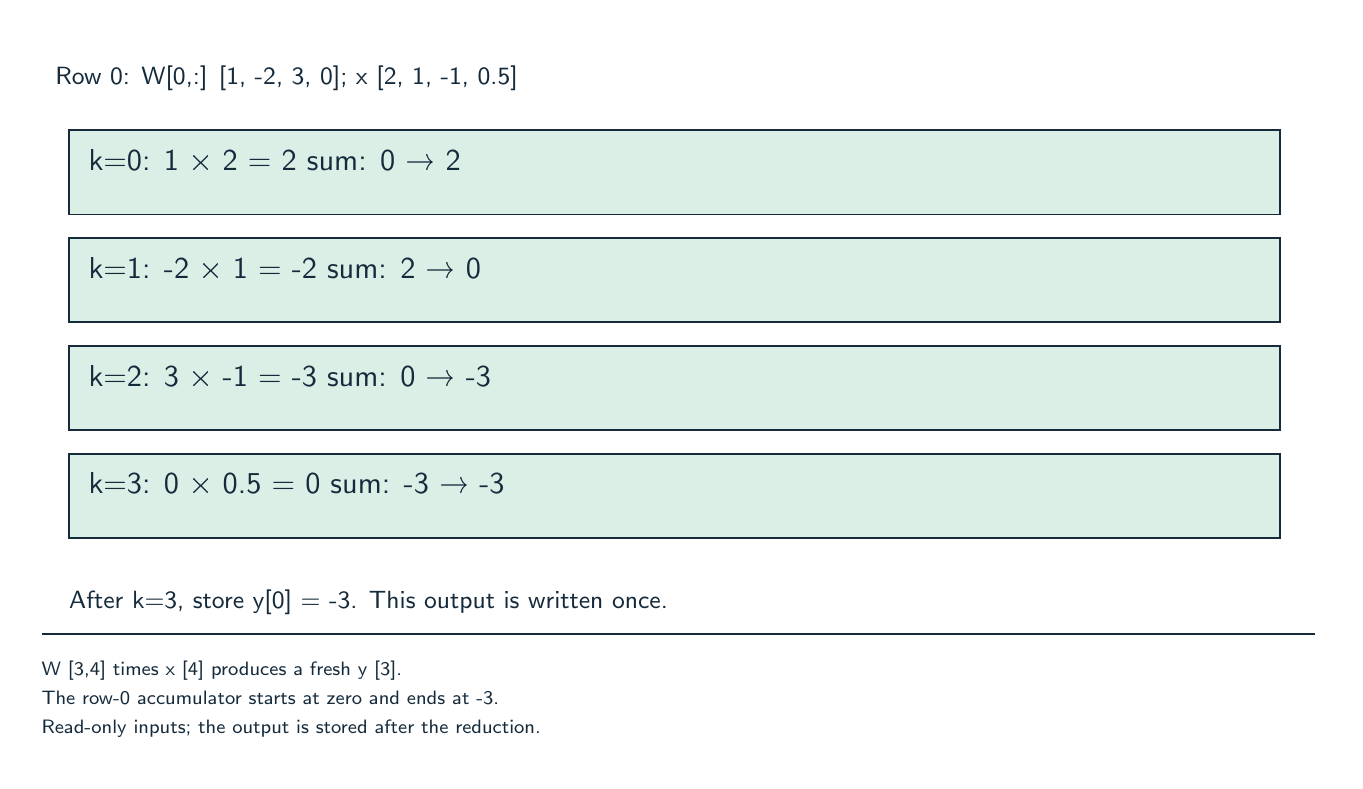
\begin{tikzpicture}[x=.5pt,y=-.5pt]
\path[use as bounding box] (30,170) rectangle (975,700);
\node[inner sep=0pt,outer sep=0pt,anchor=base west,text={rgb,255:red,21;green,43;blue,60},font=\sffamily\fontsize{9.0}{10.799999999999999}\selectfont] at (50,211) {Row 0: W[0,:] [1, -2, 3, 0]; x [2, 1, -1, 0.5]};
\path[fill={rgb,255:red,220;green,239;blue,231},draw={rgb,255:red,21;green,43;blue,60},line width=0.7pt] (60.0,244.0) rectangle (935.0,305.0);
\node[inner sep=0pt,outer sep=0pt,anchor=base west,text={rgb,255:red,21;green,43;blue,60},font=\sffamily\fontsize{10.5}{12.6}\selectfont] at (74,273) {k=0:  1 × 2 = 2     sum: 0 → 2};
\path[fill={rgb,255:red,220;green,239;blue,231},draw={rgb,255:red,21;green,43;blue,60},line width=0.7pt] (60.0,322.0) rectangle (935.0,383.0);
\node[inner sep=0pt,outer sep=0pt,anchor=base west,text={rgb,255:red,21;green,43;blue,60},font=\sffamily\fontsize{10.5}{12.6}\selectfont] at (74,351) {k=1:  -2 × 1 = -2     sum: 2 → 0};
\path[fill={rgb,255:red,220;green,239;blue,231},draw={rgb,255:red,21;green,43;blue,60},line width=0.7pt] (60.0,400.0) rectangle (935.0,461.0);
\node[inner sep=0pt,outer sep=0pt,anchor=base west,text={rgb,255:red,21;green,43;blue,60},font=\sffamily\fontsize{10.5}{12.6}\selectfont] at (74,429) {k=2:  3 × -1 = -3     sum: 0 → -3};
\path[fill={rgb,255:red,220;green,239;blue,231},draw={rgb,255:red,21;green,43;blue,60},line width=0.7pt] (60.0,478.0) rectangle (935.0,539.0);
\node[inner sep=0pt,outer sep=0pt,anchor=base west,text={rgb,255:red,21;green,43;blue,60},font=\sffamily\fontsize{10.5}{12.6}\selectfont] at (74,507) {k=3:  0 × 0.5 = 0     sum: -3 → -3};
\node[inner sep=0pt,outer sep=0pt,anchor=base west,text={rgb,255:red,21;green,43;blue,60},font=\sffamily\fontsize{9.0}{10.799999999999999}\selectfont] at (60,590) {After k=3, store y[0] = -3. This output is written once.};
\draw[fill=none,draw={rgb,255:red,21;green,43;blue,60},line width=0.75pt] (40,608) -- (960,608);
\node[inner sep=0pt,outer sep=0pt,anchor=base west,text={rgb,255:red,21;green,43;blue,60},font=\sffamily\fontsize{7.5}{9.0}\selectfont] at (40,638) {W [3,4] times x [4] produces a fresh y [3].};
\node[inner sep=0pt,outer sep=0pt,anchor=base west,text={rgb,255:red,21;green,43;blue,60},font=\sffamily\fontsize{7.5}{9.0}\selectfont] at (40,659) {The row-0 accumulator starts at zero and ends at -3.};
\node[inner sep=0pt,outer sep=0pt,anchor=base west,text={rgb,255:red,21;green,43;blue,60},font=\sffamily\fontsize{7.5}{9.0}\selectfont] at (40,680) {Read-only inputs; the output is stored after the reduction.};
\end{tikzpicture}
